\begin{table}[htb]
    \begin{center}
      \begin{tabular}{@{}rll@{}}
        \toprule
        & \multicolumn{1}{l}{\bf{Description}}
        & \multicolumn{1}{l}{\bf{Simulation values}}
        \\
        \midrule
        $\beta$
          & Transmission coefficient
          & \num{0.2}
        \\
        $\varepsilon_E$, 
        $\varepsilon_Q$,
        $\varepsilon_J$
          & Modification parameter for 
          & \num{0.3}, \num{0.0}, \num{0.1}
          \\
          &  exposed, quarantine and isolation classes 
          \\
        $\mu$
          & Natural death rate.
          & \num{0.000034}
        \\
        $\Lambda$
          & Constant recruitment rate
          & $\mu N$
        \\
        $p$
          & Net inflow of asymptomatic individuals
          & \num{0.0}
        \\
        $k_1$ 
          & Transfer rate from class 
          & \num{0.1}
          \\
          & of asymptomatic to symptomatic
          \\
        $k_2$
          & Transfer rate from the quarantine 
          & \num{0.125}
          \\ 
          & class to isolation
        \\
        \\
        $d_1$, $d_2$
          & Per-capita disease induced death rates 
          & \num{0.0079}, \num{0.0337}
          \\
          & for the symptomatic individuals and 
          \\
          & isolated individuals.
        \\
        $\sigma_1$, $\sigma_2$
          & Per-capita recovery rates for the 
          & \num{0.0337}, \num{0.0386}
          \\
          & symptomatic individuals and 
          \\
          &  isolated individuals
        \\
        \\
        $t_f$
          & Final time 
          & $\SI{1.0}{year}$
        \\
        $dt$
          & Numerical integration step size
          & \SI{1.0}{day}
        \\
          & Lower and upper bounds for $u_1$
          & \num{.05}, \num{0.5}
        \\
          & Lower and upper bounds for $u_2$
          & \num{.05}, \num{0.5}
        \\
        \\
         && \multicolumn{1}{c}{\bf{Initial conditions}}
        \\
         \cmidrule{3-3}
         && $S(0)=\num{12e6}$, $E(0)=1565$,
         \\
          && $Q(0)=292$, $I(0)=\num{695}$,
         \\
         && $J(0)=\num{326}$, $R(0)=\num{20}$
        \\
        \bottomrule
      \end{tabular}
     \caption{Parameter description for the SARS model
     \eqref{eqn:sars_model}.}
     \label{tbl:sars_table}
     \end{center}
\end{table}

\begin{figure}[htb]
  \centering
  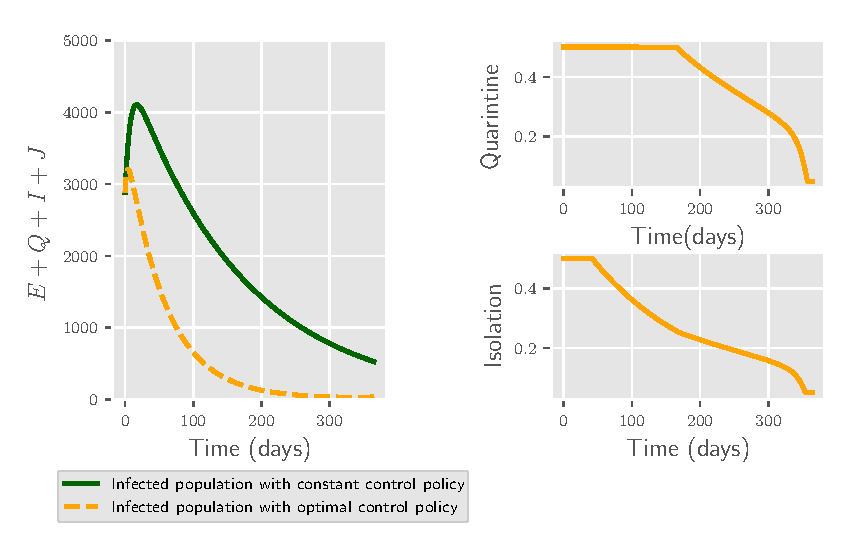
\includegraphics{Figures/figure_1_sars}
  \caption{}
  \label{fig:figure1sars}
\end{figure}

\begin{figure}[htb]
  \centering
  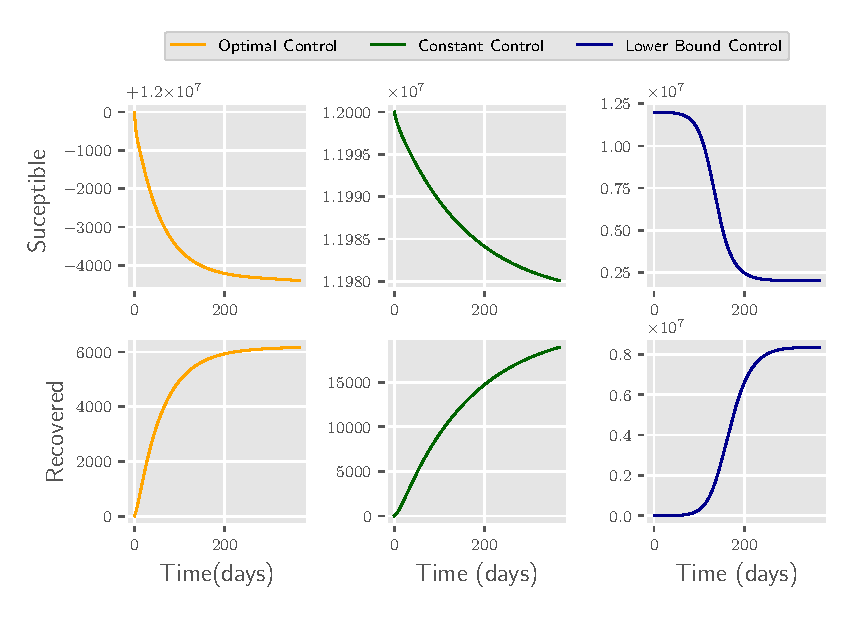
\includegraphics{Figures/figure_2_sars}
  \caption{}
  \label{fig:figure2sars}
\end{figure}

\begin{figure}[htb]
  \centering
  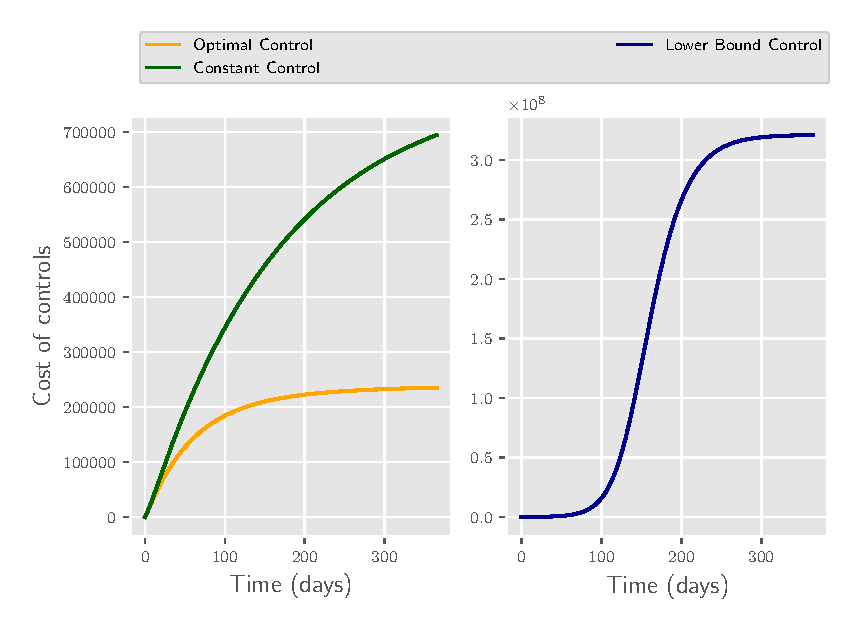
\includegraphics{Figures/figure_3_sars}
  \caption{}
  \label{fig:figure3sars}
\end{figure}